%%%%%%%%%%%%%%%%%%%%%%%%%%%%%%%%%%%%%%%%%
% Beamer Presentation
% LaTeX Template
% Version 1.0 (10/11/12)
%
% This template has been downloaded from:
% http://www.LaTeXTemplates.com
%
% License:
% CC BY-NC-SA 3.0 (http://creativecommons.org/licenses/by-nc-sa/3.0/)
%
%%%%%%%%%%%%%%%%%%%%%%%%%%%%%%%%%%%%%%%%%

%----------------------------------------------------------------------------------------
%	PACKAGES AND THEMES
%----------------------------------------------------------------------------------------

\documentclass{beamer}

\mode<presentation> {

% The Beamer class comes with a number of default slide themes
% which change the colors and layouts of slides. Below this is a list
% of all the themes, uncomment each in turn to see what they look like.

%\usetheme{default}
%\usetheme{AnnArbor}
%\usetheme{Antibes}
%\usetheme{Bergen}
%\usetheme{Berkeley}
%\usetheme{Berlin} % possivel
%\usetheme{Boadilla}
%\usetheme{CambridgeUS}
%\usetheme{Copenhagen} % possivel
%\usetheme{Darmstadt} % possivel
%\usetheme{Dresden}
%\usetheme{Frankfurt}
%\usetheme{Goettingen}
%\usetheme{Hannover}
%\usetheme{Ilmenau} % possivel
%\usetheme{JuanLesPins} % possivel
%\usetheme{Luebeck}
%\usetheme{Madrid}
%\usetheme{Malmoe}
%\usetheme{Marburg} % possivel
%\usetheme{Montpellier}
%\usetheme{PaloAlto}
%\usetheme{Pittsburgh}
%\usetheme{Rochester}
%\usetheme{Singapore}
%\usetheme{Szeged} % possivel
\usetheme{Warsaw} % igual o que o professor usa

% As well as themes, the Beamer class has a number of color themes
% for any slide theme. Uncomment each of these in turn to see how it
% changes the colors of your current slide theme.

%\usecolortheme{albatross}
%\usecolortheme{beaver} % possivel
%\usecolortheme{beetle} % possivel, pouco contraste
%\usecolortheme{crane}
%\usecolortheme{dolphin} % possivel
%\usecolortheme{dove}
%\usecolortheme{fly}
%\usecolortheme{lily}
%\usecolortheme{orchid}
%\usecolortheme{rose}
%\usecolortheme{seagull} % P&B
%\usecolortheme{seahorse}
%\usecolortheme{whale}
%\usecolortheme{wolverine}

%\setbeamertemplate{footline} % To remove the footer line in all slides uncomment this line
%\setbeamertemplate{footline}[page number] % To replace the footer line in all slides with a simple slide count uncomment this line

%\setbeamertemplate{navigation symbols}{} % To remove the navigation symbols from the bottom of all slides uncomment this line
}

\usepackage{graphicx} % Allows including images
\usepackage{booktabs} % Allows the use of \toprule, \midrule and \bottomrule in tables
\usepackage[brazilian]{babel}
\usepackage[utf8]{inputenc}
\usepackage[T1]{fontenc}
%----------------------------------------------------------------------------------------
%	TITLE PAGE
%----------------------------------------------------------------------------------------

\title[Simulação na Industria Química]{Simulação na Industria Química.\\
Termodinâmica na indústria e em simuladores }
% The short title appears at the bottom of every slide, the full title is only
% on the title page

\author{Eng. Guilherme Braganholo Flôres} % Your name
\institute[PPGEQ - UFRGS] % Your institution as it will appear on the bottom of
% every slide, may be shorthand to save space
{
UNIVERSIDADE FEDERAL DO RIO GRANDE DO SUL \\
ESCOLA DE ENGENHARIA \\
DEPARTAMENTO DE ENGENHARIA QUÍMICA \\
LAB. VIRTUAL DE PREDIÇÃO DE PROPRIEDADE \\ % Your institution for the title page
\medskip
\textit{gbflores89@gmail.com} % Your email address
} 
\date{\today} % Date, can be changed to a custom date

\begin{document}

\begin{frame}
\titlepage % Print the title page as the first slide
\end{frame}

\begin{frame}
	\frametitle{Guilherme Braganholo Flôres}
	Engenheiro Químico formado pela UFRGS
	\begin{itemize} 
		\item Universidade Federal do Rio Grande do Sul
	\end{itemize}

	Mestrando em Engenharia Química pelo PPGEQ da UFRGS
	\begin{itemize}
		\item Programa de Pós-Graduação em Engenharia Química
	\end{itemize}
 
	Área de pesquisa:
	\begin{itemize}
		\item LVPP
		\begin{itemize}
			\item Laboratório Virtual de Predição de Propriedades
		\end{itemize}
	\item Modelagem industrial 
	\item Modelos termodinâmicos
	\end{itemize}
\end{frame}


\begin{frame}
\frametitle{Sumário} % Table of contents slide, comment this block out to
% remove it
\tableofcontents % Throughout your presentation, if you choose to use
% \section{} and \subsection{} commands, these will automatically be printed on
% this slide as an overview of your presentation
\end{frame}

%------------------------------------------------------------------------------
%	PRESENTATION SLIDES
%------------------------------------------------------------------------------

\section{Introdução}
\subsection{Simuladores}
\begin{frame}
	\frametitle{Simulador de processos}
	\begin{itemize}
		\item O que é um simulador de processos?
		\item Quais os sumuladores disponives? 
		\item Como são utilizados os simuladores dentro das industrias?
		\item Quais são as vantagens do uso de simuladores?
		\item Como um simulador funciona?
		\item O que é um modelo industrial?
		\item Para que serve um modelo industrial
	\end{itemize}
\end{frame}

\begin{frame}
	\frametitle{O que são simuladores}
	\begin{columns}[c] % The "c" option specifies centered vertical alignment while
		% the "t" option is used for top vertical alignment
		\column{.5\textwidth} % Left column and width
		\begin{itemize}
			\item Qualquer programa que transforme um sistema real em um sistema de
			equações.
			\pause
			\begin{itemize}
				\item Resolvemos por cálculos feitos à mão ou por programas computacionais
			\end{itemize}
		\end{itemize}

		\column{.5\textwidth} % Right column and width
			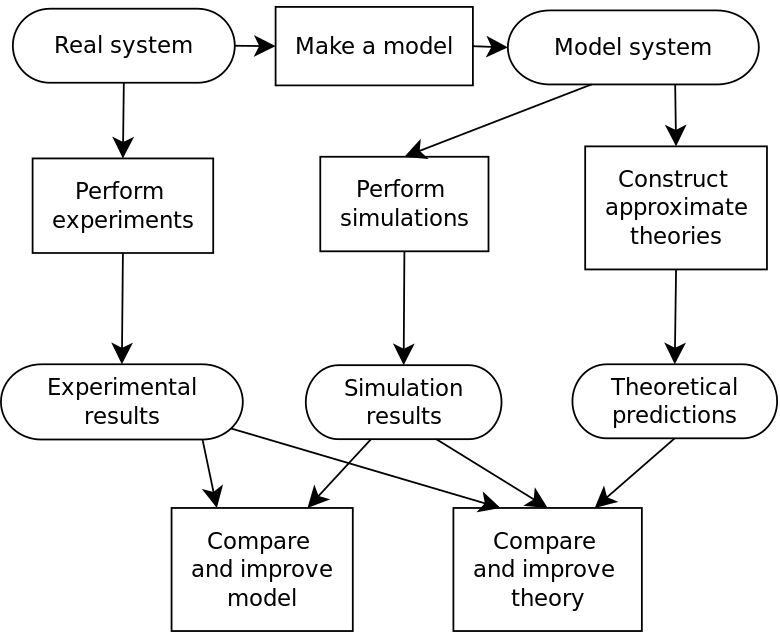
\includegraphics[width=0.95\textwidth]{img/Molecular_simulation_process.png}
	\end{columns}
\end{frame}

\begin{frame}
	\frametitle{Simuladores mais conhecidos}
	\begin{itemize}
		\item Aspen Technology --> Aspen Plus
		\item Aspen Technology --> Aspen HYSYS
		\item PSE Ltd --> gPROMS
		\item SimSci -->PRO/II
		\item \textbf{ALSOC Project --> EMSO}
		\item \textbf{VRTech --> iiSE Simulator}
	\end{itemize}
\end{frame}

\begin{frame}
	\frametitle{EMSO}
	\begin{center}
		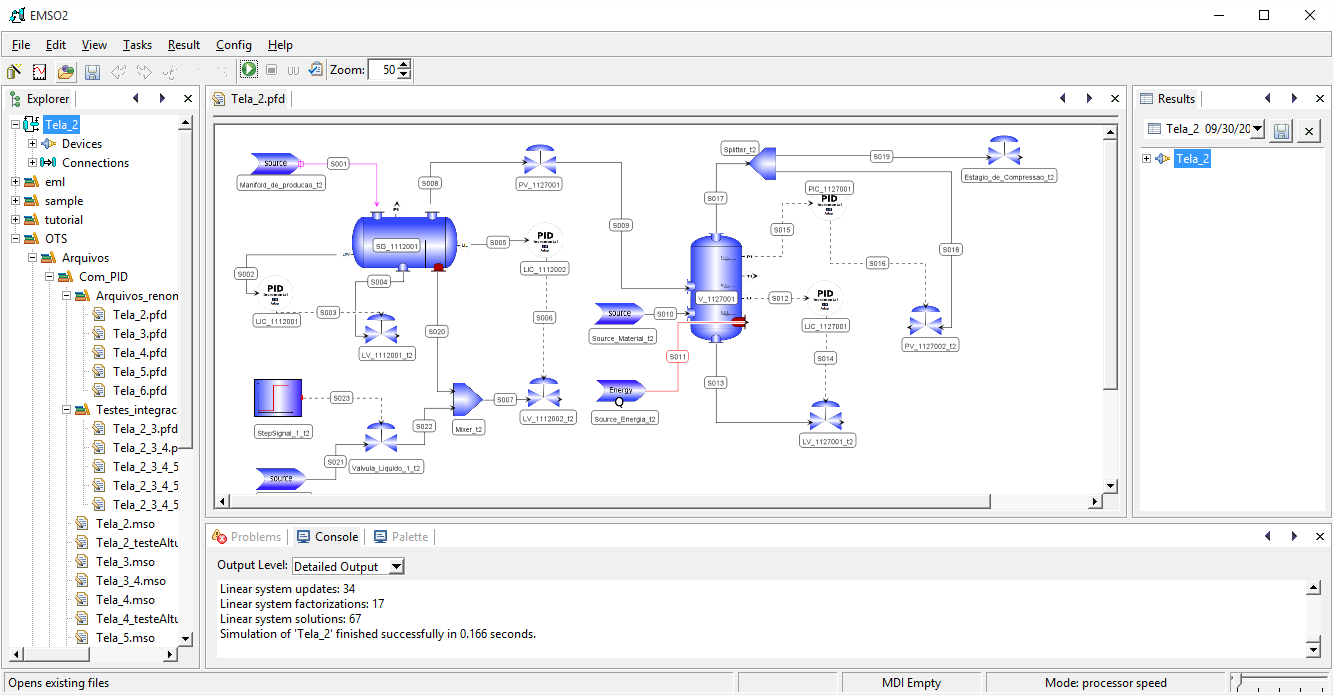
\includegraphics[width=1.0\textwidth]{img/EMSO_1.PNG}
	\end{center}
\end{frame}

\begin{frame}
	\frametitle{EMSO}
	\begin{center}
		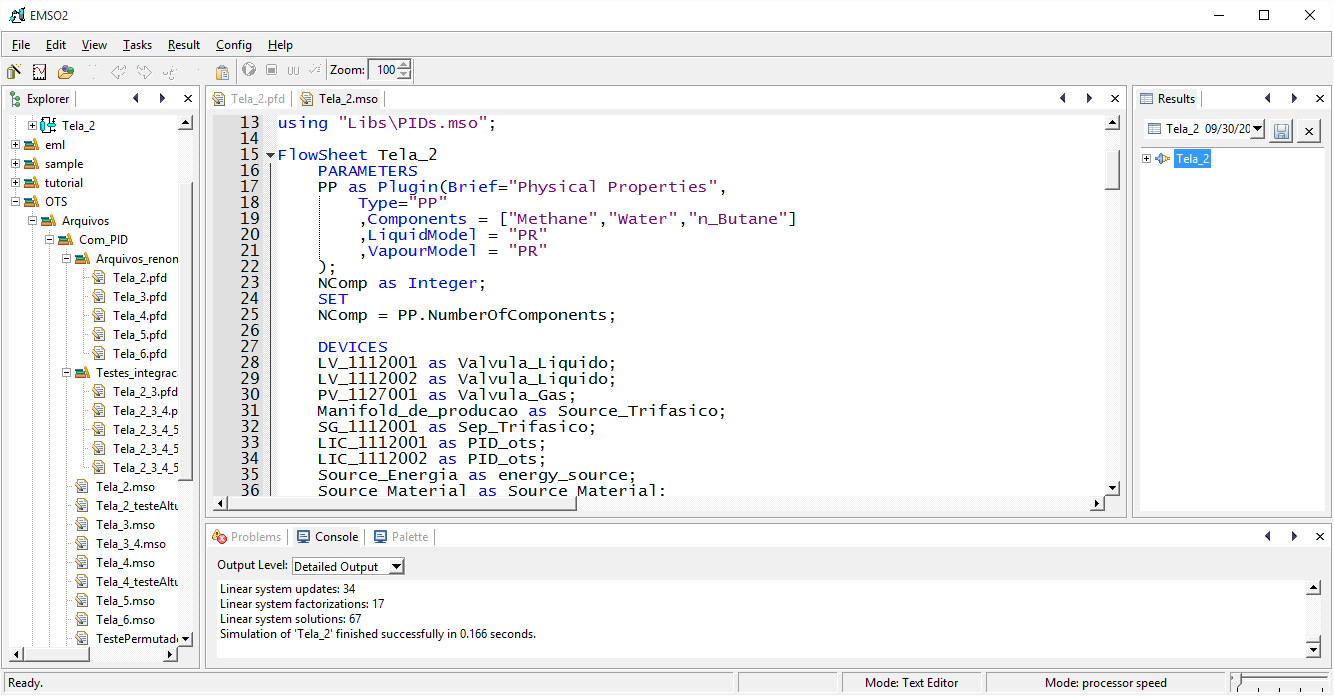
\includegraphics[width=1.0\textwidth]{img/EMSO_2.PNG}
	\end{center}
\end{frame}
 
\begin{frame}[fragile] % Need to use the fragile option when verbatim is used in the slide
\frametitle{Modelo EMSO}
	\scriptsize
	\begin{example}[Modelo de bomba simplificada em EMSO]
		\begin{verbatim}
			Model pump
			VARIABLES
				in	Inlet as stream;
				out	Outlet as streamPH;
				dP as press_delta (Brief="Pump head");
				rho as dens_mass;
			EQUATIONS
				Inlet.F = Outlet.F;
				Inlet.z = Outlet.z;
				rho * ((1-Outlet.v)/LiquidMw(Outlet.T,Outlet.P,Outlet.x) +
				Outlet.v/VapourMw(Outlet.T,Outlet.P,Outlet.y)) = 1;
				Outlet.P = Inlet.P + dP;
				Outlet.h = Inlet.h + dP/rho * sum(Mw*Inlet.z);
			end 
		\end{verbatim}
	\end{example}
\end{frame}
 
\begin{frame}
	\frametitle{Principais motivos para o uso de um simulador}
	Projeto de uma planta química

	Otimização de uma planta química

	Fazer diversos experimentos sem custo financeiro ou com custo mínimo!
		\begin{itemize}
		\item Experimentos que industrialmente são muito demorados podem ser feitos em
		questões de minutos
			\begin{itemize}
				\item Colunas de destilação podem demorar dias para entrar
				em estado estacionário
		\end{itemize}
	\end{itemize}
	
	Segurança
		\begin{itemize}
		\item Pode-se ultrapassar, sem risco os limites operacionais dos equipamentos
	\end{itemize}
\end{frame}
 
 
 
 
 
 
 
 
 
 
 
 
 
 
 
 
 
 
 
 
 
 
 
 
 
 
 
 
 
 
 
 
 
 
 
 
 
 
 
 
%------------------------------------------------

\begin{frame}
\frametitle{Bullet Points}
\begin{itemize}
\item Lorem ipsum dolor sit amet, consectetur adipiscing elit
\item Aliquam blandit faucibus nisi, sit amet dapibus enim tempus eu
\item Nulla commodo, erat quis gravida posuere, elit lacus lobortis est, quis porttitor odio mauris at libero
\item Nam cursus est eget velit posuere pellentesque
\item Vestibulum faucibus velit a augue condimentum quis convallis nulla gravida
\end{itemize}
\end{frame}

%------------------------------------------------

\begin{frame}
\frametitle{Blocks of Highlighted Text}
\begin{block}{Block 1}
Lorem ipsum dolor sit amet, consectetur adipiscing elit. Integer lectus nisl, ultricies in feugiat rutrum, porttitor sit amet augue. Aliquam ut tortor mauris. Sed volutpat ante purus, quis accumsan dolor.
\end{block}

\begin{block}{Block 2}
Pellentesque sed tellus purus. Class aptent taciti sociosqu ad litora torquent per conubia nostra, per inceptos himenaeos. Vestibulum quis magna at risus dictum tempor eu vitae velit.
\end{block}

\begin{block}{Block 3}
Suspendisse tincidunt sagittis gravida. Curabitur condimentum, enim sed venenatis rutrum, ipsum neque consectetur orci, sed blandit justo nisi ac lacus.
\end{block}
\end{frame}

%------------------------------------------------

\begin{frame}
\frametitle{Multiple Columns}
\begin{columns}[c] % The "c" option specifies centered vertical alignment while the "t" option is used for top vertical alignment

\column{.45\textwidth} % Left column and width
\textbf{Heading}
\begin{enumerate}
\item Statement
\item Explanation
\item Example
\end{enumerate}

\column{.5\textwidth} % Right column and width
Lorem ipsum dolor sit amet, consectetur adipiscing elit. Integer lectus nisl, ultricies in feugiat rutrum, porttitor sit amet augue. Aliquam ut tortor mauris. Sed volutpat ante purus, quis accumsan dolor.

\end{columns}
\end{frame}

%------------------------------------------------
\section{Second Section}
%------------------------------------------------

\begin{frame}
\frametitle{Table}
\begin{table}
\begin{tabular}{l l l}
\toprule
\textbf{Treatments} & \textbf{Response 1} & \textbf{Response 2}\\
\midrule
Treatment 1 & 0.0003262 & 0.562 \\
Treatment 2 & 0.0015681 & 0.910 \\
Treatment 3 & 0.0009271 & 0.296 \\
\bottomrule
\end{tabular}
\caption{Table caption}
\end{table}
\end{frame}

%------------------------------------------------

\begin{frame}
\frametitle{Theorem}
\begin{theorem}[Mass--energy equivalence]
$E = mc^2$
\end{theorem}
\end{frame}

%------------------------------------------------

\begin{frame}[fragile] % Need to use the fragile option when verbatim is used in the slide
\frametitle{Verbatim}
\begin{example}[Theorem Slide Code]
\begin{verbatim}
\begin{frame}
\frametitle{Theorem}
\begin{theorem}[Mass--energy equivalence]
$E = mc^2$
\end{theorem}
\end{frame}\end{verbatim}
\end{example}
\end{frame}

%------------------------------------------------

\begin{frame}
\frametitle{Figure}
Uncomment the code on this slide to include your own image from the same directory as the template .TeX file.
%\begin{figure}
%\includegraphics[width=0.8\linewidth]{test}
%\end{figure}
\end{frame}

%------------------------------------------------

\begin{frame}[fragile] % Need to use the fragile option when verbatim is used in the slide
\frametitle{Citation}
An example of the \verb|\cite| command to cite within the presentation:\\~

This statement requires citation \cite{p1}.
\end{frame}

%------------------------------------------------

\begin{frame}
\frametitle{References}
\footnotesize{
\begin{thebibliography}{99} % Beamer does not support BibTeX so references must be inserted manually as below
\bibitem[Smith, 2012]{p1} John Smith (2012)
\newblock Title of the publication
\newblock \emph{Journal Name} 12(3), 45 -- 678.
\end{thebibliography}
} 
\end{frame}

%------------------------------------------------

\begin{frame}
\Huge{\centerline{The End}}
\end{frame}

%----------------------------------------------------------------------------------------

\end{document} 